% Options for packages loaded elsewhere
\PassOptionsToPackage{unicode}{hyperref}
\PassOptionsToPackage{hyphens}{url}
%
\documentclass[
]{article}
\usepackage{amsmath,amssymb}
\usepackage{lmodern}
\usepackage{iftex}
\ifPDFTeX
  \usepackage[T1]{fontenc}
  \usepackage[utf8]{inputenc}
  \usepackage{textcomp} % provide euro and other symbols
\else % if luatex or xetex
  \usepackage{unicode-math}
  \defaultfontfeatures{Scale=MatchLowercase}
  \defaultfontfeatures[\rmfamily]{Ligatures=TeX,Scale=1}
\fi
% Use upquote if available, for straight quotes in verbatim environments
\IfFileExists{upquote.sty}{\usepackage{upquote}}{}
\IfFileExists{microtype.sty}{% use microtype if available
  \usepackage[]{microtype}
  \UseMicrotypeSet[protrusion]{basicmath} % disable protrusion for tt fonts
}{}
\makeatletter
\@ifundefined{KOMAClassName}{% if non-KOMA class
  \IfFileExists{parskip.sty}{%
    \usepackage{parskip}
  }{% else
    \setlength{\parindent}{0pt}
    \setlength{\parskip}{6pt plus 2pt minus 1pt}}
}{% if KOMA class
  \KOMAoptions{parskip=half}}
\makeatother
\usepackage{xcolor}
\usepackage[margin=1in]{geometry}
\usepackage{longtable,booktabs,array}
\usepackage{calc} % for calculating minipage widths
% Correct order of tables after \paragraph or \subparagraph
\usepackage{etoolbox}
\makeatletter
\patchcmd\longtable{\par}{\if@noskipsec\mbox{}\fi\par}{}{}
\makeatother
% Allow footnotes in longtable head/foot
\IfFileExists{footnotehyper.sty}{\usepackage{footnotehyper}}{\usepackage{footnote}}
\makesavenoteenv{longtable}
\usepackage{graphicx}
\makeatletter
\def\maxwidth{\ifdim\Gin@nat@width>\linewidth\linewidth\else\Gin@nat@width\fi}
\def\maxheight{\ifdim\Gin@nat@height>\textheight\textheight\else\Gin@nat@height\fi}
\makeatother
% Scale images if necessary, so that they will not overflow the page
% margins by default, and it is still possible to overwrite the defaults
% using explicit options in \includegraphics[width, height, ...]{}
\setkeys{Gin}{width=\maxwidth,height=\maxheight,keepaspectratio}
% Set default figure placement to htbp
\makeatletter
\def\fps@figure{htbp}
\makeatother
\setlength{\emergencystretch}{3em} % prevent overfull lines
\providecommand{\tightlist}{%
  \setlength{\itemsep}{0pt}\setlength{\parskip}{0pt}}
\setcounter{secnumdepth}{-\maxdimen} % remove section numbering
\ifLuaTeX
  \usepackage{selnolig}  % disable illegal ligatures
\fi
\IfFileExists{bookmark.sty}{\usepackage{bookmark}}{\usepackage{hyperref}}
\IfFileExists{xurl.sty}{\usepackage{xurl}}{} % add URL line breaks if available
\urlstyle{same} % disable monospaced font for URLs
\hypersetup{
  pdftitle={main},
  pdfauthor={bationoA},
  hidelinks,
  pdfcreator={LaTeX via pandoc}}

\title{main}
\author{bationoA}
\date{2023-04-08}

\begin{document}
\maketitle

\hypertarget{case-study-how-does-a-bike-share-navigate-speedy-success}{%
\section{Case Study: How does a bike-share navigate speedy
success?}\label{case-study-how-does-a-bike-share-navigate-speedy-success}}

In this case study we will work for a fictional company, Cyclistic, a
bike-share company in Chicago. For the director of marketing of the
company's, future success depends on maximizing the number of annual
memberships. Therefore, rather than creating a marketing campaign that
targets all-new customers, the director of marketing believes there is a
very good chance to convert casual riders into members.

Source:
\href{https://d3c33hcgiwev3.cloudfront.net/aacF81H_TsWnBfNR_x7FIg_36299b28fa0c4a5aba836111daad12f1_DAC8-Case-Study-1.pdf?Expires=1681084800\&Signature=WgKO~-LpPUMKTGb95H3tFbjTpbRvtu1nqBpjLACnTFrK6jBlggPYFa4lDd6jERYrYmrs7kP~4W~AJU4a3TgXhrp8XFq2c5L5gXwSIcBZNrDDKEeT1ZPXQzSUUGbFtvzy5iz-TyEvMJ-2ETjsA-oDex859GY-Ztjr8EitozVmK2w_\&Key-Pair-Id=APKAJLTNE6QMUY6HBC5A}{Link}

In order to help the company design a new marketing strategy to convert
casual riders into annual members, some questions need to be answered

\begin{itemize}
\item
  \begin{enumerate}
  \def\labelenumi{\arabic{enumi}.}
  \tightlist
  \item
    How do annual members and casual riders use Cyclistic bikes
    differently?
  \end{enumerate}
\item
  \begin{enumerate}
  \def\labelenumi{\arabic{enumi}.}
  \setcounter{enumi}{1}
  \tightlist
  \item
    Why would casual riders buy Cyclistic annual memberships?
  \end{enumerate}
\item
  \begin{enumerate}
  \def\labelenumi{\arabic{enumi}.}
  \setcounter{enumi}{2}
  \tightlist
  \item
    How can Cyclistic use digital media to influence casual riders to
    become members?
  \end{enumerate}
\end{itemize}

This case study will focus on the first question.

\hypertarget{how-do-annual-members-and-casual-riders-use-cyclistic-bikes-differently}{%
\subsection{How do annual members and casual riders use Cyclistic bikes
differently?}\label{how-do-annual-members-and-casual-riders-use-cyclistic-bikes-differently}}

\hypertarget{business-task}{%
\subsubsection{1. Business task}\label{business-task}}

The objective is to analyze and compare the usage habits of annual
members and casual riders of Cyclistic bicycles in order to identify
differences in their behavior and preferences. The goal is to gain
insights that can be used to design effective marketing strategies to
convert casual cyclists into annual members. By understanding the key
factors that influence user behavior and preferences, Cyclistic can
tailor its marketing efforts to better meet the needs of casual cyclists
and encourage them to become long-term loyal customers.

\hypertarget{description-of-data-sources}{%
\subsubsection{2. Description of data
sources}\label{description-of-data-sources}}

The data used in this study are Cyclistic's historical trip data. The
initial case study suggests to get only the previous 12 months trips
data but we will consider all data (from January 2015 to March 2023).
This could give more insights regarding changes over years.

There are several csv files containing trips data
(\href{https://divvy-tripdata.s3.amazonaws.com/index.html}{seen list
sata sets here}). The name of variables are not consistent across all
data sets but they contain similar information. The information that can
be found in these data sets are:

\begin{itemize}
\tightlist
\item
  trip\_id: ID attached to each trip taken
\item
  start\_time: day and time trip started, in CST
\item
  stop\_time: day and time trip ended, in CST
\item
  bikeid: ID attached to each bike
\item
  tripduration: time of trip in seconds
\item
  from\_station\_name: name of station where trip originated
\item
  to\_station\_name: name of station where trip terminated
\item
  from\_station\_id: ID of station where trip originated
\item
  to\_station\_id: ID of station where trip terminated
\item
  usertype: ``Customer'' is a rider who purchased a 24-Hour Pass;
  ``Subscriber'' is a rider who purchased an Annual Membership
\item
  gender: gender of rider
\end{itemize}

This project contains different files with different purpose:

\begin{itemize}
\tightlist
\item
  \href{https://github.com/bationoA/How_does_a_bike_share_navigate_speedy_success/blob/main/first_step__extraction_script.Rmd}{first\_step\_\_extraction\_script}:
  Contains scripts to download all data sets, extract and combine
  relevant csv files. The extractions scripts can easily be modify to
  download only data sets based on years. The scripts in this file
  should be the first to be ran
\item
  \href{https://github.com/bationoA/How_does_a_bike_share_navigate_speedy_success/blob/main/second_step__Formating.Rmd}{second\_step\_\_Formating}:
  To be ran at the after first\_step\_\_extraction\_script, it contains
  scripts to consolidate the format of data sets (date-time), rename
  columns or combine all data sets into only 2
\item
  \href{https://github.com/bationoA/How_does_a_bike_share_navigate_speedy_success/blob/main/third_step__Cleaning.Rmd}{third\_step\_\_Cleaning}:
  This contains scripts for cleaning the previous 2 data sets and
  combine them into one.
\item
  \href{https://github.com/bationoA/How_does_a_bike_share_navigate_speedy_success/blob/main/fourth_step__analysis.Rmd}{fourth\_step\_\_analysis}:
  This file contains scripts for all the analysis related to to case
  study
\end{itemize}

\hypertarget{summary-of-analysis}{%
\subsubsection{3. Summary of analysis}\label{summary-of-analysis}}

\textbf{Key Findings}

\begin{verbatim}
* Casual and member customers have approximately the same number of rides on weekends (Saturday and Sunday) but member customers initiate up to two times more rides than casual on working days
* Rides initiated by casual customers tend to last much longer (more than 1 to 2 times longer on average) than rides initiated by member customers
* The difference discovered in the duration of rides of cusual and member customers was tested and found significant with more than 99.99% of confidence
* The Streeter Dr & Grand Ave' station is mostly used by casual customers as starting location while the Linton St & Washington Blvd' station is mostly used by member customers
* Classic bikes are the most frequently used bikes by both customers but they all use docked bikes for longer rides
* Casual customers use classic bikes more often than member customers 
* Member customers use electric bikes more often than casual customers
\end{verbatim}

\hypertarget{in-general}{%
\paragraph{1. In general}\label{in-general}}

Comment: After removing the outliers it appears that `member'
subscription type of customers tend to use the bikes for shorter trips
compared to the `casual' customers. Let's assess the strength of this
hypothesis throught a statistical test.

\begin{figure}
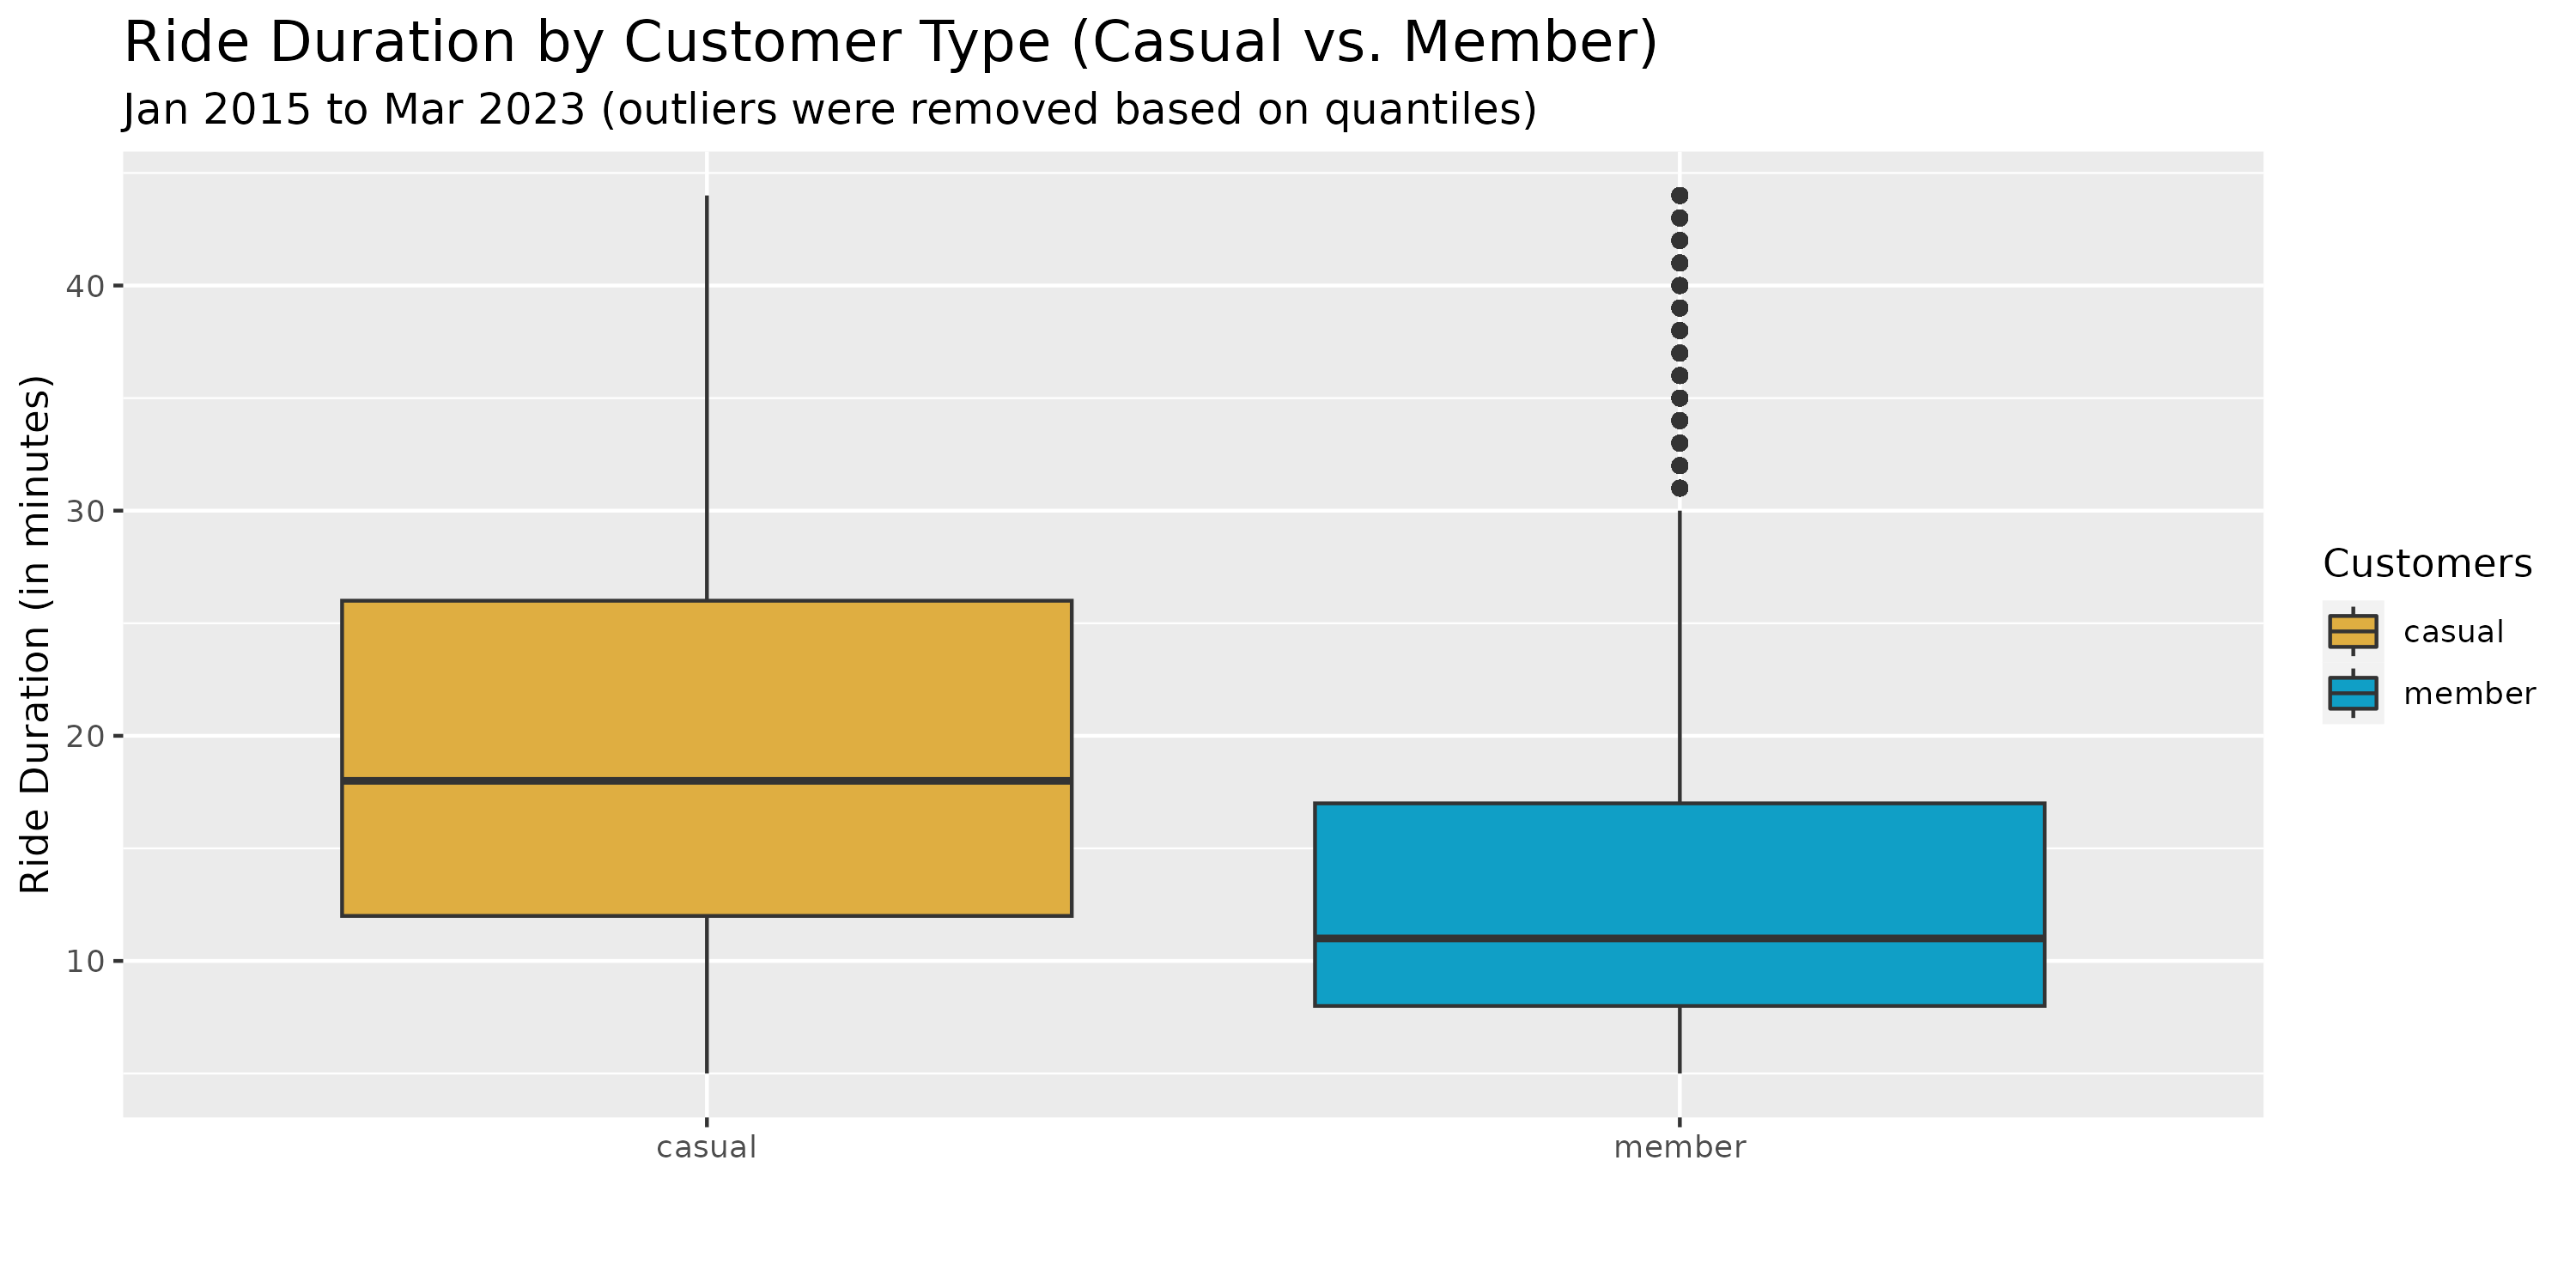
\includegraphics[width=1\linewidth]{outputs/img/box_plots__ride_duration_by_customer_type} \caption{Caption for the figure}\label{fig:fig1}
\end{figure}

\hypertarget{annual}{%
\paragraph{2. Annual}\label{annual}}

Overall, the number of bike rides each year is decreasing. However, it
is worth noting that consumers with yearly subscriptions (`members')
regularly take more bike journeys than casual customers over the course
of the study.

From 2015 to March 2023, the average trip duration for `member'
customers does not show significant variation compared to `casual'
customers. However, `casual' customers consistently use the bikes for
much longer trips than `member' customers, with trip duration ranging
from 53\% to 73\% longer. This finding could suggest that casual
customers may use the bikes for leisure or recreational purposes, while
members may use them for more utilitarian purposes such as commuting. It
also raises questions about the pricing structure and value proposition
for casual customers, who may be paying more per trip compared to
members but may not be utilizing the service as frequently. Further
analysis of customer behavior and preferences could provide insights
into potential strategies for increasing casual customer engagement and
loyalty.

\begin{figure}
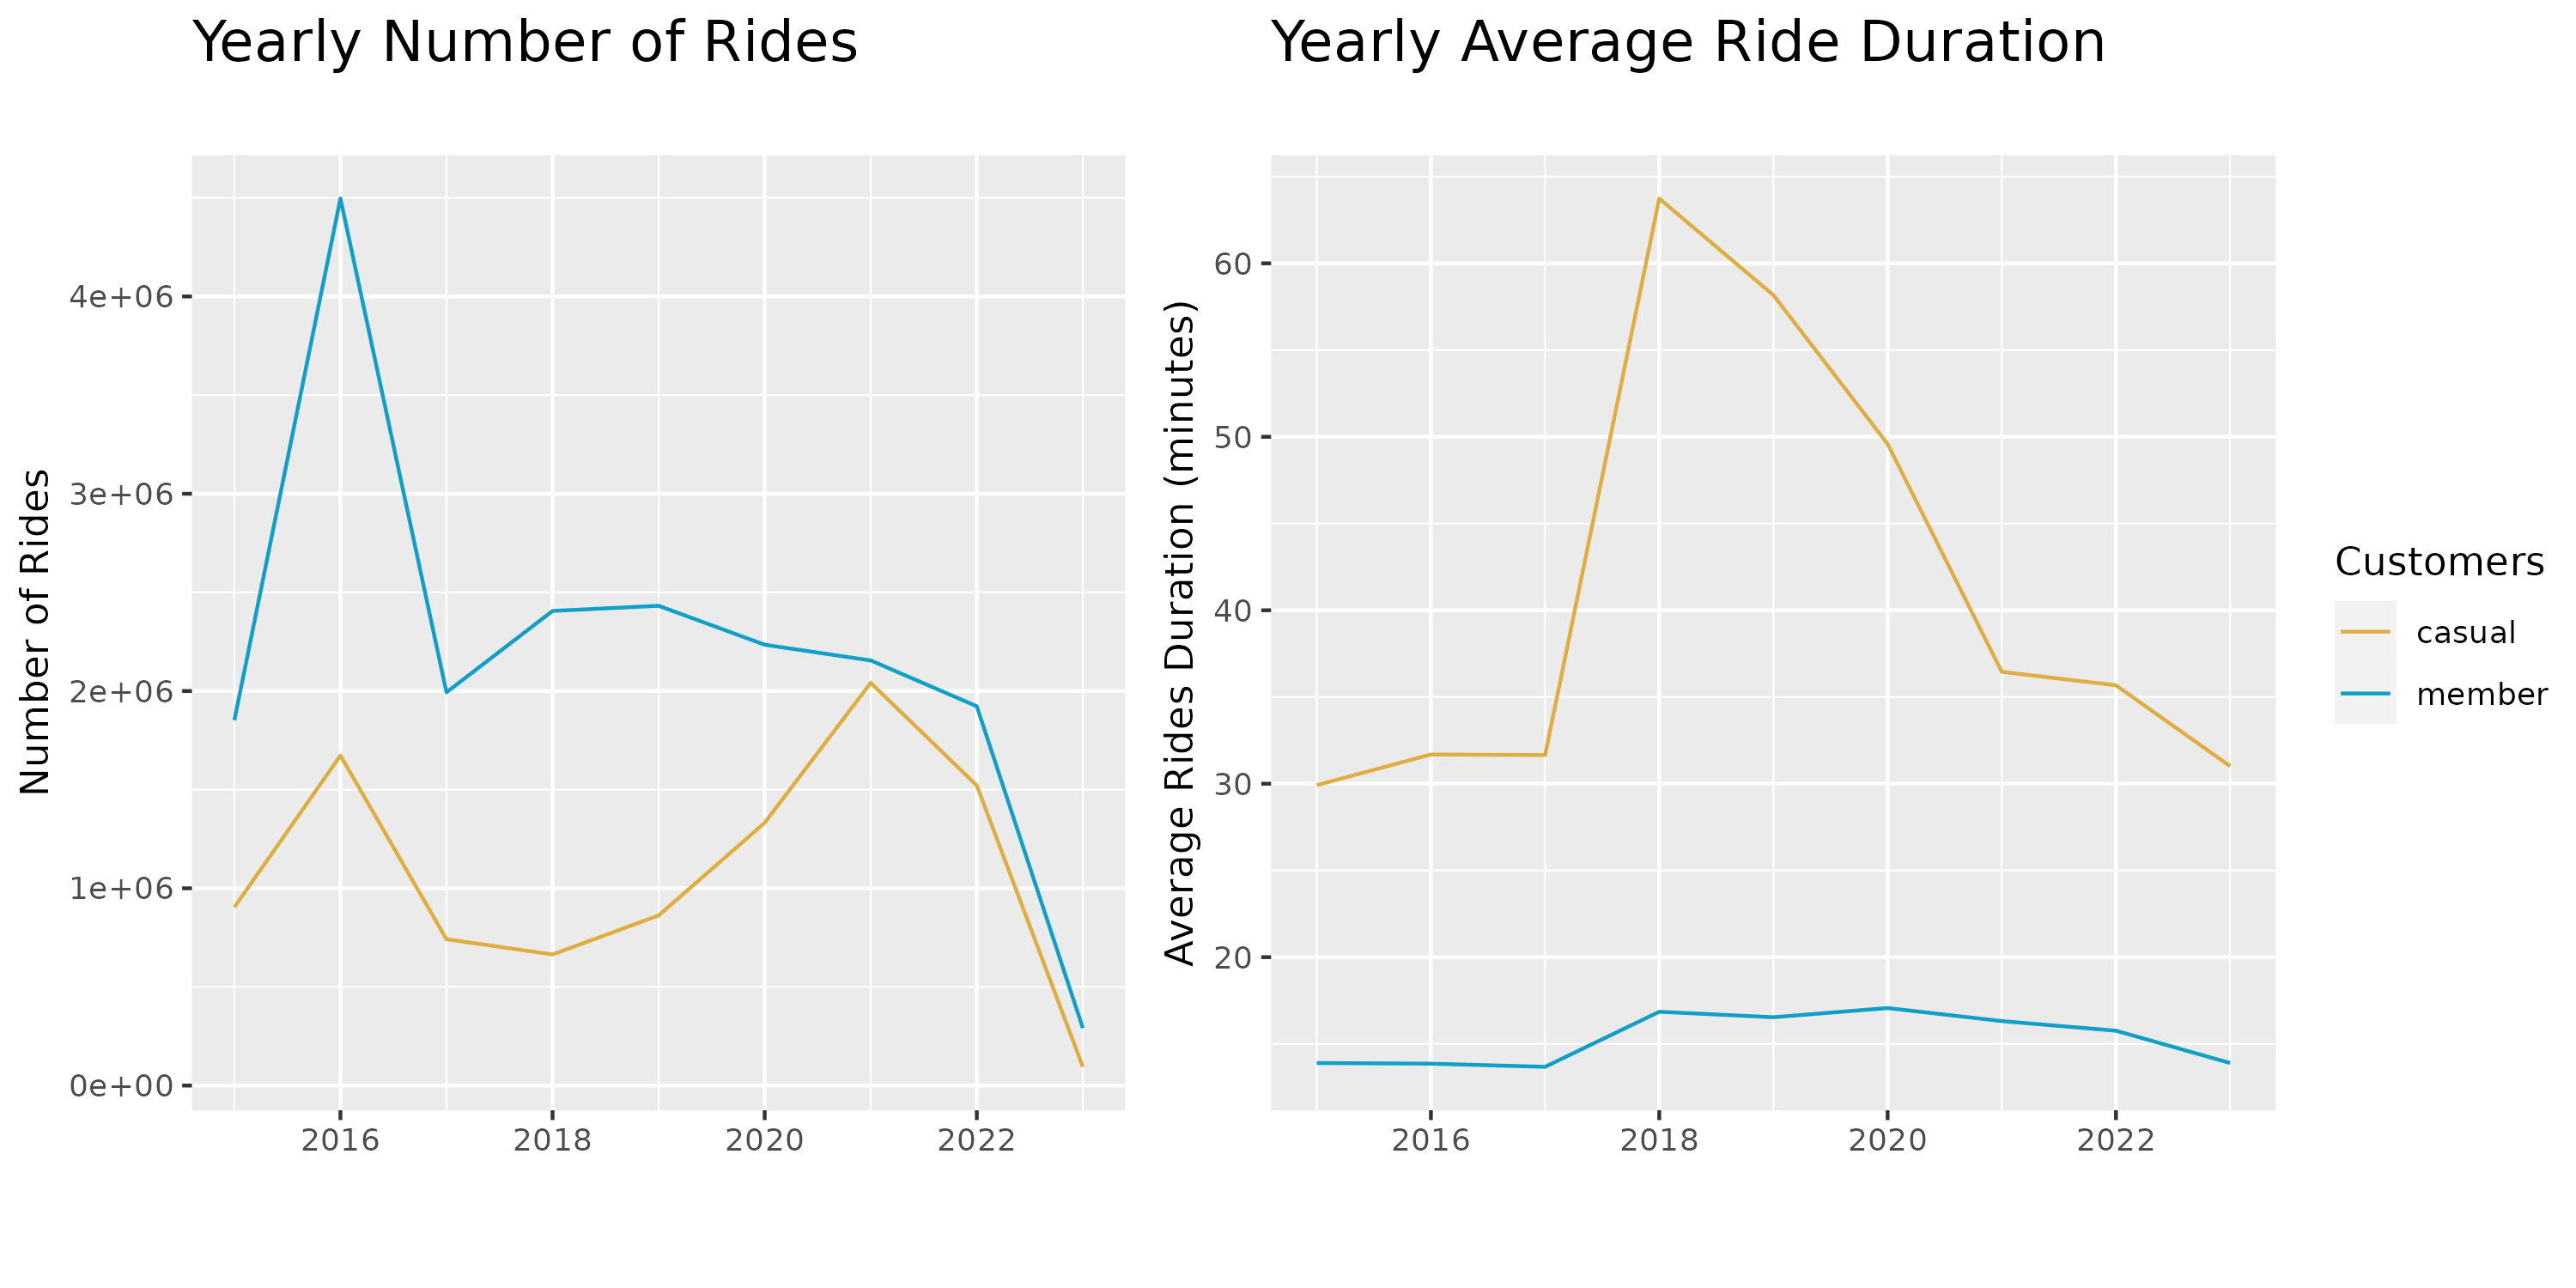
\includegraphics[width=1\linewidth]{outputs/img/line_plots__average_number_of_rides_and_duration_per_customer_by_year} \end{figure}

\hypertarget{monthly}{%
\paragraph{3. Monthly}\label{monthly}}

Comment: The number of bike rides for each type of customer appears to
be normally distributed over the months. However, there is a clear trend
that annual subscribers (`member') have been taking more bike trips per
month compared to casual customers since 2015.

Comment: Based on the data, it appears that there is a significant
difference in the average trip duration between casual customers and
annual subscribers (`member') on a monthly basis. Despite a slight
decrease in the average duration over time, casual customers
consistently take longer bike trips compared to annual subscribers.

Comment: The average time spent for monthly trips by casual customers is
more than the double of the average time spent by member customers.

\begin{figure}
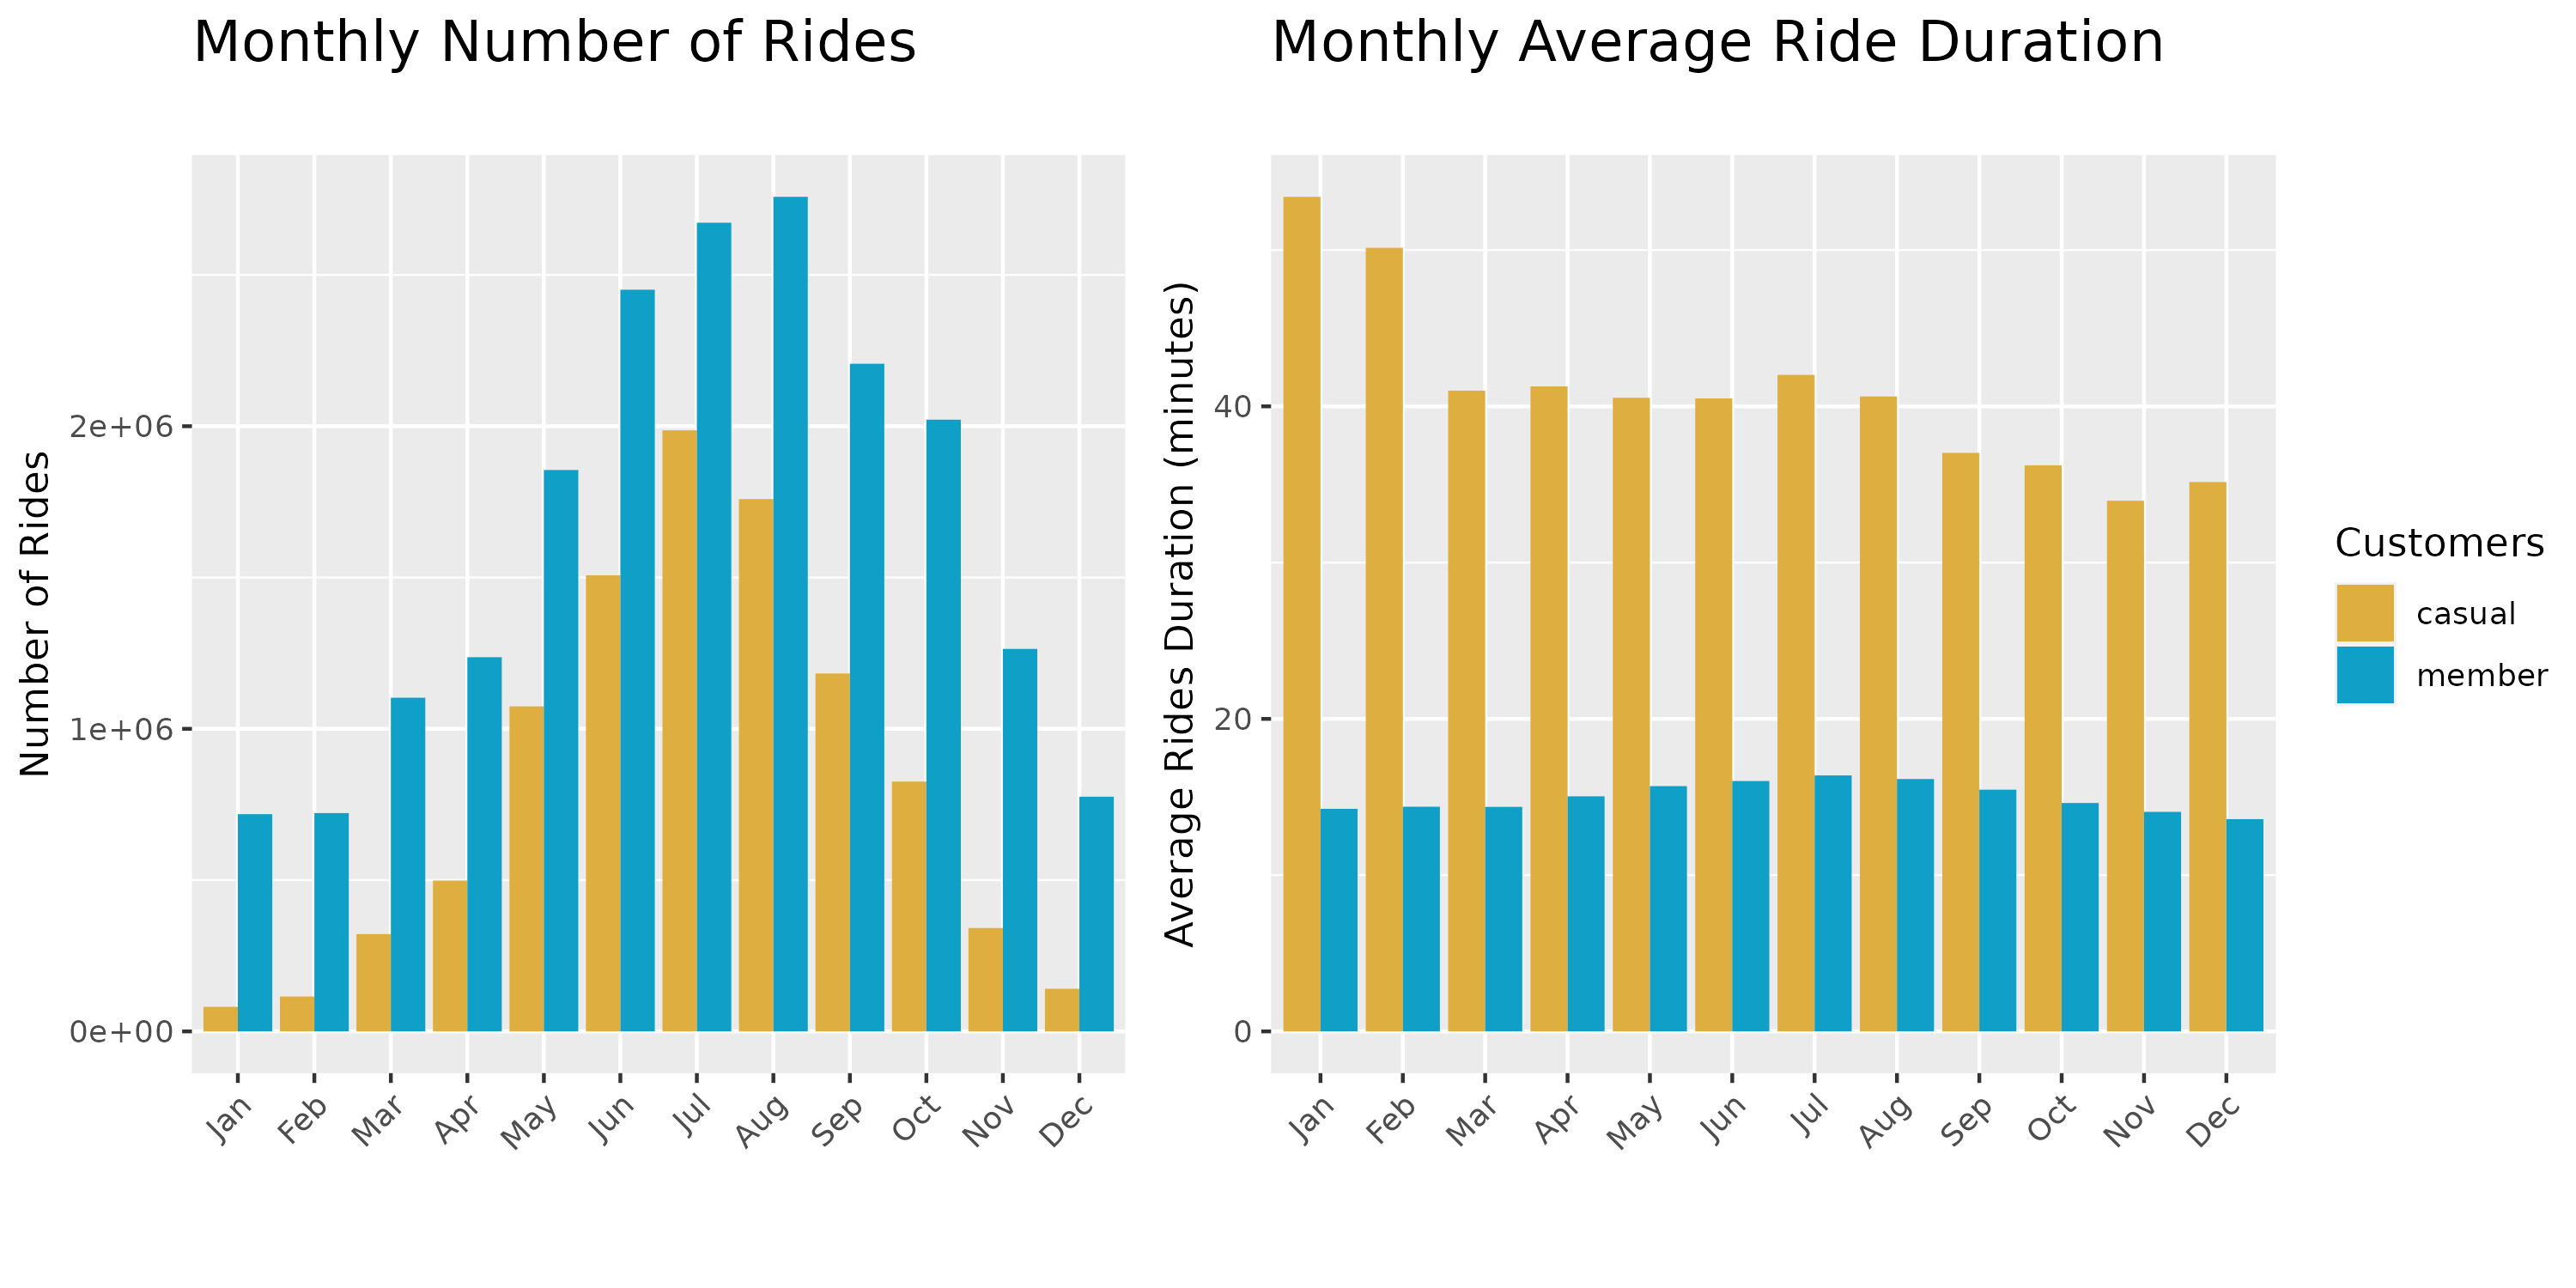
\includegraphics[width=1\linewidth]{outputs/img/bar_plots__average_number_of_rides_and_duration_per_customer_by_month} \end{figure}

\hypertarget{daily}{%
\paragraph{4. Daily}\label{daily}}

Comment: Casual and member customers tend to use bikes at the same rate
during weekends (Saturday and Sunday). However, during working days,
member customers use the bikes 1 to 2 times more frequently than casual
customer.

Comment: From 2015 to March 2023, casual customers have been using the
bikes for longer than member customers

Comment: The average time spent for daily trips by casual customers is
more than the double of the average time spent by member customers.

\begin{figure}
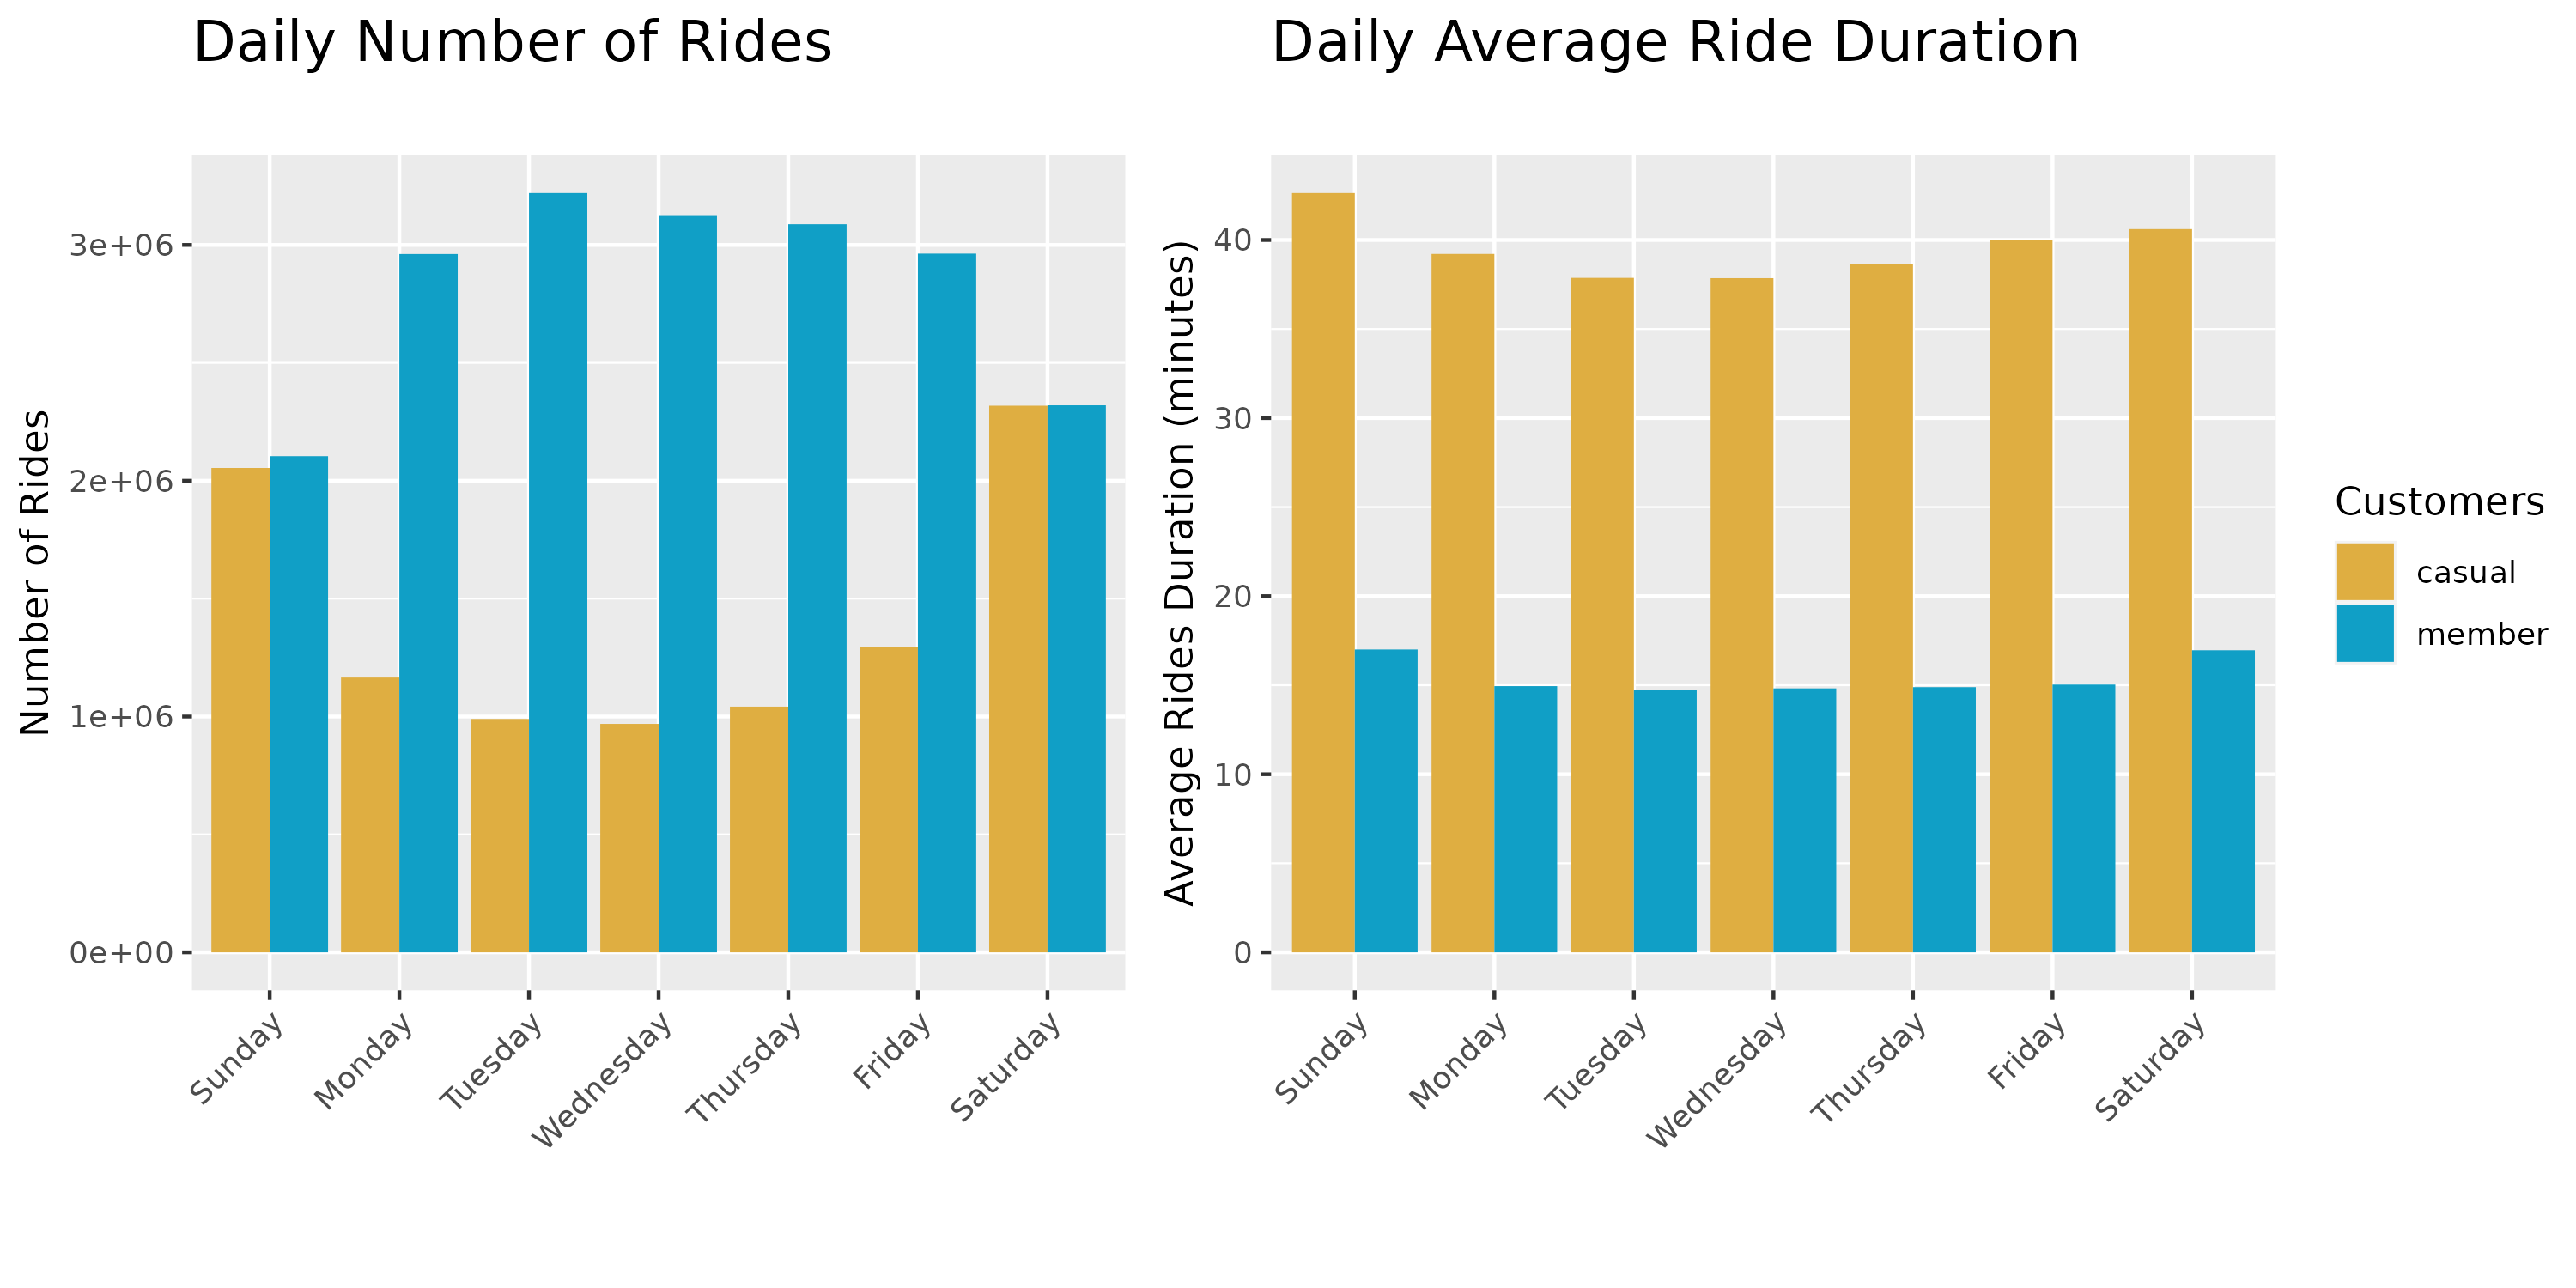
\includegraphics[width=1\linewidth]{outputs/img/bar_plots__average_number_of_rides_and_duration_per_customer_by_day} \end{figure}

\hypertarget{testing-the-difference-of-trips-duration-between-casual-and-member-customers}{%
\paragraph{5. Testing the difference of trips duration between casual
and member
customers}\label{testing-the-difference-of-trips-duration-between-casual-and-member-customers}}

From the above analysis it appeared that a clear difference exists
between casual and member customers when it comes to the duration of
their rides. In this section we'll use statistical tests to evaluate the
significance of this difference. The tests will be on central trends
such as means or medians.

The question we're trying to answer here is: Is there a significant
difference in the duration of the trips between the two categories of
customers (casual and member)? The results of different tests conducted
are summarized in the bellow table.

\begin{longtable}[]{@{}
  >{\raggedright\arraybackslash}p{(\columnwidth - 8\tabcolsep) * \real{0.2895}}
  >{\raggedright\arraybackslash}p{(\columnwidth - 8\tabcolsep) * \real{0.5263}}
  >{\raggedleft\arraybackslash}p{(\columnwidth - 8\tabcolsep) * \real{0.0316}}
  >{\raggedright\arraybackslash}p{(\columnwidth - 8\tabcolsep) * \real{0.0842}}
  >{\raggedright\arraybackslash}p{(\columnwidth - 8\tabcolsep) * \real{0.0684}}@{}}
\caption{Test Results}\tabularnewline
\toprule()
\begin{minipage}[b]{\linewidth}\raggedright
Test
\end{minipage} & \begin{minipage}[b]{\linewidth}\raggedright
H0
\end{minipage} & \begin{minipage}[b]{\linewidth}\raggedleft
Alpha
\end{minipage} & \begin{minipage}[b]{\linewidth}\raggedright
P\_value
\end{minipage} & \begin{minipage}[b]{\linewidth}\raggedright
Reject\_H0
\end{minipage} \\
\midrule()
\endfirsthead
\toprule()
\begin{minipage}[b]{\linewidth}\raggedright
Test
\end{minipage} & \begin{minipage}[b]{\linewidth}\raggedright
H0
\end{minipage} & \begin{minipage}[b]{\linewidth}\raggedleft
Alpha
\end{minipage} & \begin{minipage}[b]{\linewidth}\raggedright
P\_value
\end{minipage} & \begin{minipage}[b]{\linewidth}\raggedright
Reject\_H0
\end{minipage} \\
\midrule()
\endhead
Levene - Homogeneity of variance & variance in casual group is equal
(statistically) to variance in member group & 0.05 & p-value \textless{}
1e-05 & Yes (99.99\%) \\
Shapiro - normality of distribution - casual customers & The data are
normally distributed & 0.05 & p-value \textless{} 1e-05 & Yes
(99.99\%) \\
Shapiro - normality of distribution - member customers & The data are
normally distributed & 0.05 & p-value \textless{} 1e-05 & Yes
(99.99\%) \\
T-Test - Equality of means & averages trips duration for casual and
member customers are not statistically different & 0.05 & p-value
\textless{} 1e-05 & Yes (99.99\%) \\
Wilcoxon rank-sum test - Equality of medians & median value of trips
duration for `casual' and `member' customers are not statistically
different & 0.05 & p-value \textless{} 1e-05 & Yes (99.99\%) \\
\bottomrule()
\end{longtable}

We've decided to run a T-Test (Student test) to compare the average trip
duration of casual and member customers.

First, we ran a homogeneity of variance test to check if the variances
of the data were not statistically different in both groups. The result
was not in our favor, and we had to reject the null hypothesis with more
than 99.99\% confidence. Next, we ran a normality test, which showed
that the duration of the rides for both categories was not normally
distributed. The results of these these two violate the
\href{fourth_step__analysis.Rmd}{assumptions of a T-Test}. These
violations of assumptions were taken into account before proceeding with
the T-Test.

Despite the violated assumptions, we decided to conduct a T-Test, which
resulted in rejecting the null hypothesis with more than 99.99\%
confidence. This means that there is a statistically significant
difference in the average duration of trips between the two categories
of customers. However, it was crucial to note that the assumptions for
the T-Test were violated, therefore alternative tests are needed to add
credit to this conclusion.

Finally, we decided to go for a non-parametric test (no assumptions are
required) called the Wilcoxon rank-sum, which tests the equality of
medians. The result was in our favor as we had to reject the null
hypothesis with more than 99.99\% confidence. Thus, we concluded that
the difference in the duration of trips between casual and member
customers was statistically significant, regardless of the type of test
used.

\hypertarget{top-5-starting-stations-by-customers-type-members-vs-casual-users}{%
\paragraph{6. Top 5 starting stations by customers type (members vs
casual
users)}\label{top-5-starting-stations-by-customers-type-members-vs-casual-users}}

There is a clear difference between casual and member customers in terms
of starting station. Most casual riders start their trips at the
Streeter Dr \& Grand Ave' station (457,718 trips), with more than 2
times the number of started rides by member customers (124,443 trips).
In the other hand member customers mostly go to the Clinton St \&
Washington Blvd' station to pick up a bike for their trip. However their
number of rides (278,769 trips) less differ from the one of casual
customers as it is just 0.92 times higher than the number of rides of
casual customers.

\begin{figure}
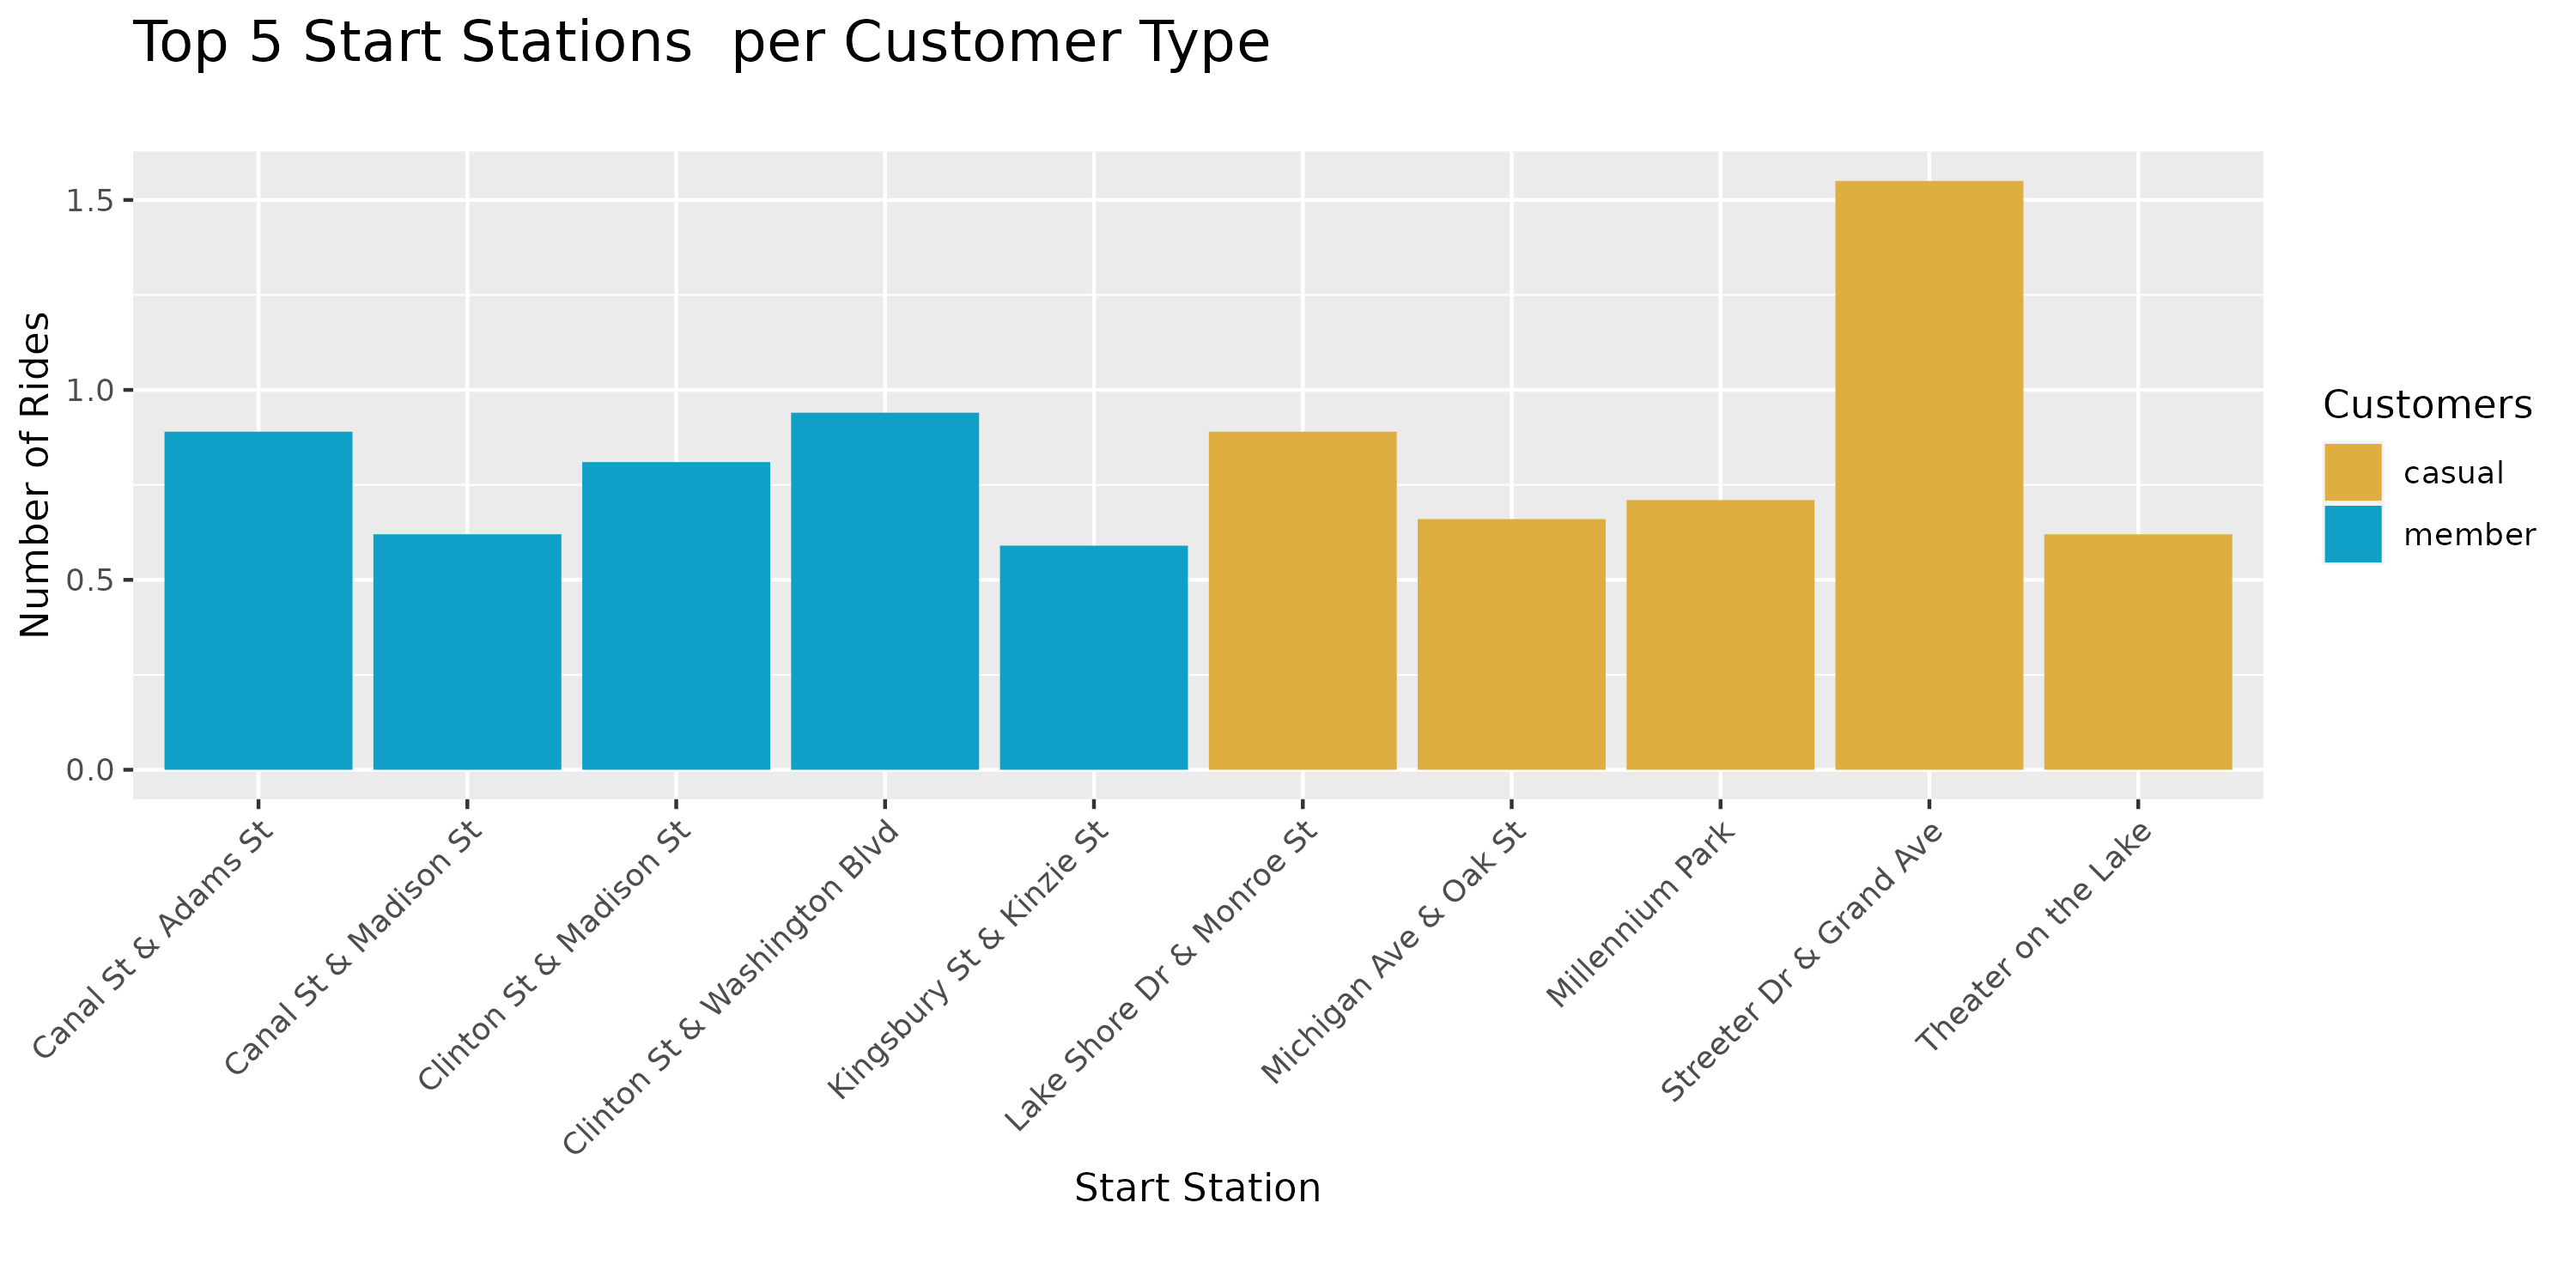
\includegraphics[width=1\linewidth]{outputs/img/bar_chart__number_of_rides_per_customer_by_top_5_start_station} \end{figure}

\hypertarget{bikes-preference-by-customers-type}{%
\paragraph{7. Bikes preference by customers
type}\label{bikes-preference-by-customers-type}}

number of rides and duration per bikes type and customers

\hypertarget{recommendations-for-an-effective-marketing-strategy}{%
\subsubsection{4. Recommendations for an effective marketing
strategy}\label{recommendations-for-an-effective-marketing-strategy}}

Based on the results of the analysis, here are nine recommendations for
designing marketing strategies aimed at converting casual riders into
annual members:

\begin{itemize}
\item
  \textbf{1. Offer promotions and discounts for annual memberships
  during weekdays}: Member customers tend to use the bikes more often.
  This can encourage casual riders to become members and take advantage
  of the benefits of more frequent rides during weekdays.
\item
  \textbf{2. Promote the benefits of annual membership for weekend
  riders}: Although casual and member customers have similar number of
  rides during weekends, annual members have more flexibility to take
  longer trips without worrying about extra fees. Marketing campaigns
  should emphasize this benefit to encourage casual riders to become
  annual members.
\item
  \textbf{3. Offer incentives to encourage casual riders to use docked
  bikes more often}: Since casual riders account for the majority of
  trips made with docked bikes, incentives such as discounts or free
  rides can encourage them to become more loyal customers and
  potentially convert to annual members.
\item
  \textbf{4. Focus marketing efforts on promoting the benefits of using
  bikes from different starting stations}: Since casual customers tend
  to use a specific starting station much more often, marketing
  campaigns should focus on the benefits of exploring different areas
  and using bikes from different starting stations. This can encourage
  casual riders to become more adventurous and potentially become annual
  members.
\item
  \textbf{5. Highlight the cost savings of annual memberships for
  frequent riders}: The analysis shows that casual riders tend to use
  bikes for longer duration than annual members. Promoting the cost
  savings of an annual membership for frequent riders can encourage
  casual riders to become members and take advantage of the cost savings
  for longer trips.
\item
  \textbf{6. Offer membership trial periods}: The company can offer
  casual riders the chance to try out the annual membership for a
  certain period of time (e.g.~a week or a month) to see if they would
  benefit from the service. This can help to increase the number of
  annual members by giving casual riders a chance to experience the
  benefits of an annual membership without committing to it fully.
\item
  \textbf{7. Create a community for annual members}: Since annual
  members tend to be more frequent users of the service, the company can
  create a community for them to promote social interaction and
  encourage them to use the service more often. This can help to
  increase their loyalty to the service and encourage casual riders to
  convert to annual members.
\end{itemize}

\hypertarget{for-further-analysis}{%
\subsubsection{5. For further analysis}\label{for-further-analysis}}

Further data collection analysis can be conducted in order to have a
better understanding of the customers and increase annual subscription
while providing a better service to customers:

\begin{itemize}
\tightlist
\item
  Conduct a quick survey to understand more the reason to of choosing
  (or not) annual subscription and what they use the bikes for.
\item
  Conduct a neighborhood analysis around different stations as well as
  between start and end stations?
\end{itemize}

\end{document}
